\section{Câu a: Thiết kế và sinh dữ liệu}
\label{sec:a}

\subsection{Thuộc tính và lý do lựa chọn}
Mười bốn thuộc tính đầu vào phản ánh năm khía cạnh: lịch sử mua hàng, giá trị chi tiêu, mức dùng khuyến mãi, hành vi duyệt và mức tương tác với nền tảng, cộng với đặc điểm khách.
\var{customer_id} chỉ là khóa và bị loại khỏi mọi ma trận đặc trưng.

\begin{table}[htbp]
\centering\small
\caption{Data Dictionary rút gọn (bản đầy đủ gồm phân phối dự kiến và lý do chọn nằm ở \var{data_dictionary.csv}).}
\label{tab:dict}
\begin{tabularx}{\linewidth}{llllX}
\toprule
Thuộc tính & Nhóm & Kiểu & Miền & Ý nghĩa\\
\midrule
\var{age} & Nhân khẩu & số nguyên & 18--70 & Tuổi (phân biệt yếu có chủ đích)\\
\var{n_orders_12m} & Mua hàng & số nguyên & $\ge 1$ & Số đơn 12 tháng gần nhất\\
\var{avg_order_value} & Chi tiêu & thực & $>0$ (USD) & Giá trị đơn trung bình\\
\var{total_spend_12m} & Chi tiêu & thực & $>0$ (USD) & Tổng chi 12 tháng ($\approx$ số đơn $\times$ giá trị đơn; cố ý đa cộng tuyến)\\
\var{recency_days} & Mua hàng & số nguyên & 0--365 & Số ngày từ đơn gần nhất\\
\var{discount_usage_rate} & Khuyến mãi & thực & $[0,1]$ & Tỉ lệ đơn dùng mã giảm giá\\
\var{sessions_per_month} & Tương tác & thực & $\ge 0{,}5$ & Số phiên truy cập mỗi tháng\\
\var{avg_session_minutes} & Tương tác & thực & 1--90 & Thời lượng phiên trung bình\\
\var{pages_per_session} & Duyệt & thực & 1--60 & Số trang sản phẩm xem mỗi phiên\\
\var{cart_abandon_rate} & Duyệt & thực & $[0,1]$ & Tỉ lệ giỏ hàng bị bỏ\\
\var{membership_tier} & Thứ tự & thứ tự & bronze$<$silver$<$gold & Hạng thành viên\\
\var{device_type} & Định danh & định danh & 3 mức & Thiết bị chính\\
\var{preferred_category} & Định danh & định danh & 5 mức & Ngành hàng ưa thích\\
\var{app_installed} & Nhị phân & nhị phân & 0/1 & Đã cài ứng dụng\\
\bottomrule
\end{tabularx}
\end{table}

\subsection{Cơ chế sinh dữ liệu giả lập}
Dữ liệu được sinh theo mô hình nhiều tầng để các thuộc tính có quan hệ nhân quả hợp lý thay vì là các con số độc lập:
\begin{enumerate}
\item \textbf{Phân khúc ẩn} (4 nhóm, kích thước $48/78/66/68$): khách giá trị cao (\emph{HighValue}), săn khuyến mãi (\emph{PromoHunter}), mua không thường xuyên (\emph{Infrequent}) và chủ yếu duyệt (\emph{Browser}).
Khoảng 18\% khách là ``cầu nối'': hành vi pha giữa phân khúc của họ và một phân khúc khác, tạo độ chồng lấn có chủ đích.
\item \textbf{Bốn đặc điểm ẩn liên tục}: gắn bó $E$, ý định mua $I$, mức chi mỗi đơn $W$, nhạy cảm giá $S$, lấy từ phân phối chuẩn nhiều chiều quanh trung bình của phân khúc (có tương quan trong cụm).
\item \textbf{Thuộc tính quan sát} sinh theo phương trình nghiệp vụ ($\sigma$ là hàm logistic, $\varepsilon_i$ là nhiễu riêng):
\end{enumerate}
\begin{align*}
\mathrm{sessions} &= \exp(a_0 + a_1 E + \varepsilon_1),\\
\mathrm{n\_orders} &\sim \mathrm{NegBin}\!\big(\text{trung bình } 12\cdot\mathrm{sessions}\cdot\sigma(c_0 + c_1 I + \varepsilon_2)\big)\quad(\ge 1),\\
\mathrm{abandon} &= \sigma(b_0 - b_1 I + \varepsilon_3), \qquad \mathrm{discount} = \sigma(g_0 + g_1 S + \varepsilon_4),\\
\mathrm{AOV} &= \exp(m_0 + m_1 W + \beta_{\mathrm{cat}} - m_2\,\mathrm{discount} + \varepsilon_5),\\
\mathrm{total} &= \mathrm{n\_orders}\cdot\mathrm{AOV}\cdot e^{\varepsilon_6}, \qquad \mathrm{recency} \sim \mathrm{Gamma}\!\big(\text{trung bình } \tfrac{365}{\mathrm{n\_orders}+1}\,e^{-0{,}3E}\big),\\
\mathrm{tier} &= \text{cắt ngưỡng}\big(\ln \mathrm{total} + \varepsilon_7\big).
\end{align*}
Thiết bị, ngành hàng và cài ứng dụng được lấy mẫu theo phân khúc, tuổi và mức gắn bó. Hệ quả: các cặp (số đơn, tổng chi), (số phiên, số trang) tương quan mạnh; mức dùng khuyến mãi làm giảm giá trị đơn; hạng thành viên suy từ tổng chi nhưng không tất định.

\subsection{Nhiễu, ngoại lai và giá trị thiếu}
Ba loại vấn đề được thêm tuần tự lên dữ liệu sạch D0, lưu thành bốn file đối chiếu (D0 \var{data_clean_reference}, D1 \var{data_after_noise}, D2 \var{data_after_outliers}, D3 \var{data_raw_corrupted}) cùng một nhật ký ghi từng ô được chủ động thay đổi (1.040 ô nhiễu, 42 ô ngoại lai, 65 ô thiếu).

\begin{table}[htbp]
\centering\small
\caption{Cơ chế thêm nhiễu, ngoại lai và giá trị thiếu.}
\label{tab:corrupt}
\begin{tabularx}{\linewidth}{lX}
\toprule
Loại & Cách tạo (và cơ sở nghiệp vụ)\\
\midrule
Nhiễu D0$\to$D1 (mọi dòng, 4 cột số) &
\var{avg_order_value}: nhân lognormal $\sigma = 0{,}12$ (quy đổi tiền, làm tròn); \var{recency_days}: cộng $\mathcal N(0, 4^2)$ ngày (lệch múi giờ);
\var{avg_session_minutes}: nhân lognormal $\sigma = 0{,}15$; \var{sessions_per_month}: cộng $\mathcal N(0, 1{,}5^2)$. Kỳ vọng không đổi (sai lệch trung bình $<1{,}8\%$), có chặn biên.\\
Ngoại lai D1$\to$D2 (15 khách khác nhau) &
\textbf{8 hợp lệ}: 3 ``cá voi'' (nhiều đơn và đơn lớn), 2 đại lý mua sỉ, 2 mua một lần món giá trị lớn, 1 duyệt cực đoan; cường độ đặt theo hàng rào Tukey của D1 và nhất quán nghiệp vụ (không quá 1 đơn/phiên).
\textbf{7 lỗi}, mỗi khách hỏng đúng một ô: \var{age}=150, \var{recency_days}=$-12$, \var{discount_usage_rate}=1,8, \var{avg_order_value} gấp 100 lần,
\var{avg_session_minutes}=1440, \var{cart_abandon_rate}=1,35, \var{sessions_per_month}=999 (mã sentinel).\\
Thiếu D2$\to$D3 (số ô chính xác) &
\var{age}: MCAR 8\% (21 ô); \var{avg_session_minutes}: MAR theo \var{device_type} (desktop 18\%, tablet 15\%, mobile 7\%), 12\% (31 ô); \var{preferred_category}: MCAR 5\% (13 ô). Ô đã mang ngoại lai không bị xóa.\\
\bottomrule
\end{tabularx}
\end{table}

\subsection{Kiểm tra nghiệm thu và hiệu chỉnh}
Script sinh dữ liệu tự kiểm tra 42 ràng buộc (đạt 42/42): đúng $N$, số thuộc tính, số ô thiếu, nhiễu không thiên lệch, đúng 15 khách ngoại lai và không ô nào bị xóa, dữ liệu D0 nhất quán nghiệp vụ,
tái lập (md5 giống hệt giữa các lần chạy), nhãn ẩn không có mặt trong file dữ liệu.

Độ khó của bài toán được hiệu chỉnh \emph{chỉ trên dữ liệu sạch D0} và trước khi xem kết quả xử lý nhiễu. Hai lần đầu đều sai: thiết kế ban đầu quá dễ (K-Means đạt ARI $0{,}98$,
sẽ gây hiệu ứng trần ở câu e), mô hình nhân quả đầu tiên lại quá khó (ARI $0{,}47$). Cấu hình cuối cho ARI của K-Means trên D0 bằng $0{,}73$ (hạt giống chính) và $0{,}71\pm0{,}05$ (10 hạt giống sinh mới);
độ chính xác của cây quyết định chỉ dùng một thuộc tính tốt nhất là $0{,}68$ ($<0{,}70$, ngưỡng đặt trước), tức không thuộc tính đơn lẻ nào quyết định phân khúc.
Hai lỗi của cách tạo ngoại lai được phát hiện và sửa: hai ``đại lý'' ban đầu không phải cực trị thống kê, và một ``cá voi'' có 309 đơn/năm với 36 phiên/tháng (phi nghiệp vụ; bộ kiểm tra tự động không bắt được, phải đọc nhật ký mới thấy).

\begin{figure}[htbp]
\centering
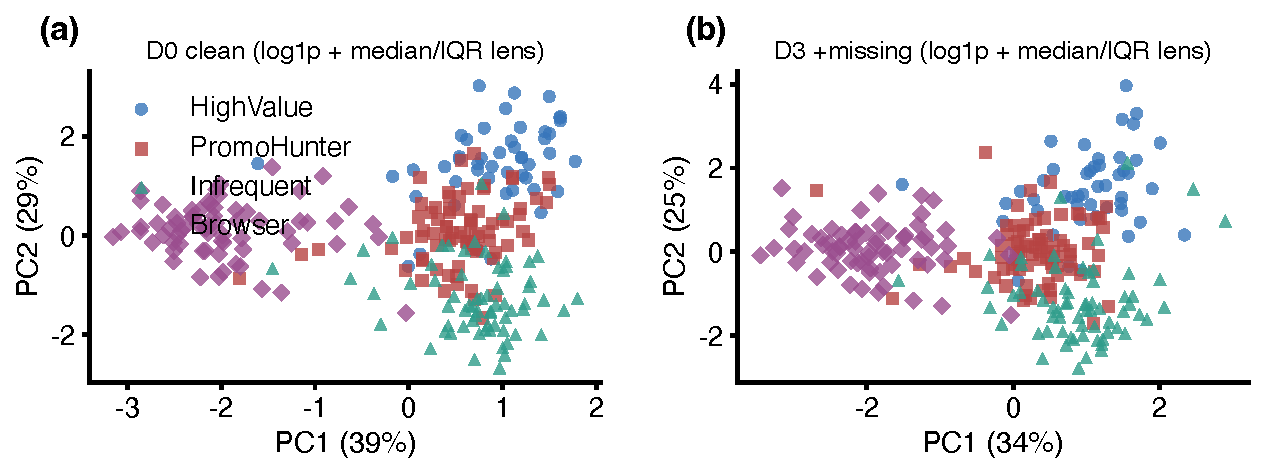
\includegraphics[width=\linewidth]{fig17_pca_hidden_segments.pdf}
\caption{Cấu trúc phân khúc ẩn trên không gian PCA 2 chiều (cùng cách biểu diễn log1p, median/IQR; chỉ để chẩn đoán). (a) Dữ liệu sạch D0: bốn nhóm tách được nhưng chồng lấn do khách ``cầu nối''.
(b) D3 sau khi thêm nhiễu, ngoại lai và giá trị thiếu: cấu trúc bị méo và các nhóm trộn nhiều hơn.}
\label{fig:a_pca}
\end{figure}

\subsection{Giả định của cơ chế sinh}
\begin{itemize}
\item Bốn đặc điểm ẩn, các phương trình và mọi hệ số do chúng tôi đặt, không rút từ dữ liệu thật; không mô hình hóa thời gian hay mùa vụ; mỗi khách có ít nhất một đơn trong năm.
\item Nhiễu độc lập giữa các cột; cơ chế thiếu MCAR/MAR được giả định, không suy ra từ dữ liệu thật.
\item Một sai khác so với thiết kế đã thống nhất: bỏ phụ thuộc ``mức dùng khuyến mãi giảm theo hạng gold'' vì tạo vòng lặp (hạng suy từ tổng chi, tổng chi suy từ khuyến mãi).
\end{itemize}
\FloatBarrier
